
\documentclass[pdflatex,sn-mathphys-num]{sn-jnl}


\usepackage{graphicx}%
\usepackage{subcaption}%
\usepackage{multirow}%
\usepackage{amsmath,amssymb,amsfonts}%
\usepackage{amsthm}%
\usepackage{mathrsfs}%
\usepackage[title]{appendix}%
\usepackage{xcolor}%
\usepackage{textcomp}%
\usepackage{manyfoot}%
\usepackage{booktabs}%
\usepackage{algorithm}
% \usepackage{algorithmic}%
\usepackage{algorithmicx}
\usepackage{algpseudocode}
\usepackage{listings}%

\usepackage{tikz}
\usetikzlibrary{shapes.geometric, shapes.misc, arrows.meta, positioning}




%% as per the requirement new theorem styles can be included as shown below
\theoremstyle{thmstyleone}%
\newtheorem{theorem}{Theorem}
\newtheorem{proposition}{Proposition}%
\newtheorem{remark}{Remark}
\newtheorem{lemma}{Lemma}
\newtheorem{definition}{Definition}
\newtheorem{corollary}{Corollary}
\newtheorem{example}{Example}



\raggedbottom
%%\unnumbered% uncomment this for unnumbered level heads

\begin{document}

\title{From Topological Design to Screening-Ready MOF Candidate Models: Symmetry-Aware Enumeration and Reconstruction}

\author[]{\fnm{Hui} \sur{Li}}

\author[]{\fnm{Jing} \sur{Tian}}

\author[]{\fnm{Dahuan} \sur{Liu}}

\author[]{\fnm{Minman} \sur{Tong}}

\author[]{\fnm{Qingyuan} \sur{Yang}}

\affil[]{\orgname{Beijing University of Chemical Technology}, \city{Beijing}, \postcode{100029}, \country{China}}


\abstract{
Metal-organic frameworks (MOFs) are modular porous crystals whose properties can be tuned by changing metal nodes, organic linkers, topology, and component ordering. This tunability makes MOF design a large combinatorial problem, where redundant candidates can consume screening effort before any atomistic evaluation begins. Existing construction, identification, and screening workflows do not by themselves define an orientation-compatible quotient of fixed-net ordered assignments. Here we couple proper-rotation enumeration with Kabsch-based rigid-body reconstruction to generate one representative per symmetry-distinct assignment and carry it forward as an oriented periodic model.% 中文翻译：金属有机框架（MOF）是模块化多孔晶体，其性质可通过改变金属节点、有机连接体、拓扑和组分排布来调控。这种可调性使 MOF 设计成为大规模组合问题，其中冗余候选会在原子级评估开始前消耗筛选资源。已有构建、识别和筛选工作流本身并不定义固定网络有序指派中与取向相容的取商方式。本文将真旋转枚举与基于 Kabsch 的刚体重构相耦合，为每个对称互异指派生成一个代表元，并将其转化为具有取向信息的周期模型。


In representative nets, exhaustive degree-constrained spaces with up to $\sim\!5\times10^{5}$ configurations are enumerated in seconds, and orbit counts agree with Burnside and CASM checks. In a sampled \texttt{ffc}/\texttt{fjh} reconstruction audit, all 27 tested assignments produced sanitizable, topology-consistent, and clash-free periodic starting models. Fixed-composition DFT calculations and CO$_2$/N$_2$ screening examples show that the reconstructed models can be directly used in downstream scoring. For rigid or semi-rigid building units, the workflow thus provides a traceable route from fixed-net assignment spaces to crystal-level starting models suitable for subsequent validation.%在代表性网络中，规模最高约为 $\sim\!5\times10^{5}$ 个构型的可穷举度约束空间可在数秒内完成枚举，轨道计数与 Burnside 及 CASM 校验一致。在抽样的 \texttt{ffc}/\texttt{fjh} 重构审计中，全部 27 个受试指派均生成了可清理、拓扑一致且无碰撞的周期性起始模型。固定组成 DFT 计算和 CO$_2$/N$_2$ 筛选示例表明，重构模型可直接用于下游打分。对于刚性或半刚性构建单元，该工作流由此提供了一条从固定网络指派空间到适用于后续验证的晶体级起始模型的可追踪路线。

}

\keywords{Metal-Organic Frameworks; Crystal Engineering; Candidate Generation; Geometric Reconstruction; Symmetry-Constrained Screening}

\pacs[MSC Classification]{05A10, 01A05}

\maketitle

\section*{Introduction}
\label{sec:intro}
Metal-organic frameworks (MOFs) are studied for gas storage, catalysis, and separation because their pore structures and chemical functions can be varied~\cite{zhou2012introduction,furukawa2013chemistry}. This same modularity creates a design problem: a finite library of nodes and linkers can generate millions of hypothetical frameworks~\cite{wilmer2012large}. High-throughput computational screening (HTCS), often combined with machine learning, is used to select candidates for further study~\cite{colon2014high, park2024data, kim2025machine}. The useful candidate set must be broad enough to sample chemical space, compact enough to avoid redundant simulations, and concrete enough for structure-based evaluation.
% 中文翻译：金属有机框架（MOF）因孔结构和化学功能可调，被用于气体储存、催化和分离等研究~\cite{zhou2012introduction,furukawa2013chemistry}。同样的模块化也形成了设计问题：有限的节点和连接体库即可生成数百万种假设框架~\cite{wilmer2012large}。高通量计算筛选（HTCS）常与机器学习结合，用于筛选后续研究候选~\cite{colon2014high, park2024data, kim2025machine}。有用的候选集合既要足以采样化学空间，又要紧凑到避免冗余模拟，并且必须具体到能接受结构层面评估。

Several method classes already support this process. ToBaCCo constructs hypothetical MOFs from selected nets and building units by manipulating net embeddings and then optimizing geometries~\cite{colon2017topologically}. MOFid and MOFkey identify and deconstruct MOF structures for search and cheminformatics analysis~\cite{bucior2019identification}. Data-driven work from the Snurr, Rosen, Smit, and Kulik communities has advanced large-scale screening, inverse design, diversity analysis, and stability prediction~\cite{colon2014high,bucior2019identification,yao2021inverse,moosavi2020diversity,nandy2021stable}. Recent language-model, flow-based, and free-energy models further address generative or downstream scoring tasks~\cite{niyongabo2025freeenergy,badrinarayanan2025mofgpt,Kim2024MOFFlowFM}. These approaches define important parts of the design pipeline. They leave a narrower combinatorial step: for a fixed embedded net and a degree-compatible building-unit library, decide which ordered assignments are related by admissible rotations and should therefore share one representative.
% 中文翻译：已有多类方法支撑这一过程。ToBaCCo 通过调节网络嵌入并优化几何，从选定网络和构建单元构建假想 MOF~\cite{colon2017topologically}。MOFid 和 MOFkey 用于 MOF 结构的识别、拆分、检索和化学信息学分析~\cite{bucior2019identification}。来自 Snurr、Rosen、Smit 和 Kulik 等团队的数据驱动工作推动了大规模筛选、逆向设计、多样性分析和稳定性预测~\cite{colon2014high,bucior2019identification,yao2021inverse,moosavi2020diversity,nandy2021stable}。近期语言模型、基于流的模型和自由能模型进一步处理生成或下游打分任务~\cite{niyongabo2025freeenergy,badrinarayanan2025mofgpt,Kim2024MOFFlowFM}。这些方法定义了设计流程中的重要环节，但仍留下一个更窄的组合问题：对于固定嵌入网络和配位数相容的构建单元库，判断哪些有序指派可由允许的旋转互相联系，因而应共享同一个代表元。

This step is important in multivariate and digital reticular chemistry. In multivariate MOFs, function can depend on both component identities and their arrangement over crystallographic positions or local sequences~\cite{zhang2015multivariate,helal2017multivariate,ji2020sequencing,canossa2023sequences}. Digital reticular chemistry treats such choices as variables in automated searches across reticular chemical space~\cite{lyu2020digital}. Before relaxation or property prediction, the same composition on the same net can therefore correspond to many ordered candidates. Non-redundant enumeration is needed to keep the genuinely distinct arrangements while removing copies generated by the net symmetry.
% 中文翻译：这一步在多变量和数字网状化学中尤为重要。在多变量 MOF 中，功能可能同时取决于组分身份，以及这些组分在晶体学位置或局部序列中的排布~\cite{zhang2015multivariate,helal2017multivariate,ji2020sequencing,canossa2023sequences}。数字网状化学把这类选择作为网状化学空间自动搜索中的变量~\cite{lyu2020digital}。因此，在弛豫或性质预测之前，同一网络和同一组成仍可能对应多个有序候选。无冗余枚举的作用是保留真正互异的排布，同时去除由网络对称性产生的重复副本。

We solve this fixed-net problem by formulating building-unit assignment as coloring on a quotient graph. The proper-rotation group $\Gamma$ acts on the independent sites, and each orbit represents one symmetry-distinct ordered assignment. A subgroup-lattice descent algorithm visits fixed-point spaces from high-symmetry strata to the identity layer, while degree pools and composition counts prune infeasible branches. Because fixed-point spaces can overlap, complete colorings are canonicalized over the full group before insertion into a global representative set. The result is one retained assignment per proper-rotation orbit.
% 中文翻译：本文通过把构建单元指派表述为商图着色来解决这一固定网络问题。真旋转群 $\Gamma$ 作用在独立位点上，每条轨道代表一个对称互异的有序指派。子群格下降算法从高对称层级到恒等层依次访问不动点空间，并用配位数构建单元库和组成计数剪除不可行分支。由于不同不动点空间可能重叠，完整着色在插入全局代表元集合之前会在完整群 $\Gamma$ 下正则化。所得结果是每个真旋转轨道只保留一个指派。

The retained representative is then carried into rigid-body reconstruction. Secondary building units (SBUs) and linkers have connection geometry, directionality, and possible handedness, so the symmetry reduction must remain compatible with the placement step. We therefore use proper rotations as the default equivalences; improper operations are included only when the building-unit library is known to be invariant under them. Kabsch alignment then maps each accepted assignment to an oriented periodic model.
% 中文翻译：保留的代表元随后进入刚体重构。次级构建单元（SBU）和连接体具有连接几何、方向性以及可能的手性，因此对称约化必须与后续放置步骤保持相容。因此，本文默认只使用真旋转作为等价操作；只有当构建单元库已知对相应非真操作不变时，才纳入非真操作。随后，Kabsch 对齐把每个被接受的指派映射为具有取向信息的周期模型。

Deterministic symmetry-constrained enumeration is already well developed for substitutional disorder in inorganic crystals~\cite{mckay1998isomorph, mckay2014practical, hart2008algorithm, hart2009generating, hart2012generating, morgan2017generating}. We use these ideas in a reticular setting where the enumerated graph assignments are carried forward into oriented framework models. This coupling of orbit enumeration and geometric reconstruction distinguishes the workflow from substitutional enumeration on an isotropic lattice.
% 中文翻译：针对无机晶体中的替位无序，确定性的对称约束枚举已经发展得较为成熟~\cite{mckay1998isomorph, mckay2014practical, hart2008algorithm, hart2009generating, hart2012generating, morgan2017generating}。本文在网状化学场景中使用这些思想，其中被枚举的图指派会继续进入具有取向信息的框架模型。轨道枚举与几何重构的耦合，是该流程区别于各向同性晶格替位枚举的关键。

The study therefore tests a complete fixed-net route: non-redundant assignment generation, oriented reconstruction, and downstream screening on the resulting periodic models. The CIFs are traceable pre-relaxation candidates within specified design spaces. Their role is to connect controlled topological assignments to crystal-level validation, not to claim final materials discovery before relaxation or property testing.
% 中文翻译：因此，本文检验的是一条完整的固定网络路线：无冗余指派生成、有取向重构，以及在所得周期模型上的下游筛选。所得 CIF 是指定设计空间内可追踪的弛豫前候选。它们的作用是把受控拓扑指派连接到晶体层面的验证，而不是在弛豫或性质测试之前宣称最终材料发现。

\section*{Candidate Generation and Reconstruction}

\subsection*{Organizing Non-Redundant Candidate Generation}
\label{sec:theory}
We formulate candidate generation as coloring on a quotient graph. The topological design input is a chosen net, degree-typed building-unit pools, and optional composition counts. Factoring lattice translations leaves the unique primitive-cell sites, and each coloring assigns a degree-compatible building unit to each site. The reduced space is finite, but it still grows rapidly and contains many symmetry-equivalent assignments.
% 中文翻译：我们把候选生成表述为商图着色问题。拓扑设计输入包括所选网络、按配位数分类的构建单元库和可选组成计数。扣除晶格平移后，只保留初基胞中的独立位点；每种着色把配位数相容的构建单元分配到各位点。该空间有限，但仍会快速增长，并包含大量对称等价指派。

The workflow is sketched in Fig.~\ref{fig:pipeline}. It quotients the design space by the proper-rotation group $\Gamma$, the finite set of orientation-preserving rotations acting on quotient-graph sites. This choice keeps enumeration compatible with oriented reconstruction. Improper operations can be added only when the building-unit library is known to be invariant under them.
% 中文翻译：该流程见图~\ref{fig:pipeline}。本文按真旋转群 $\Gamma$ 对设计空间取商，即作用在商图位点上的有限保取向旋转集合。这一选择使枚举与有取向重构相容。只有当构建单元库已知对某些非真操作不变时，才将这些操作加入等价规则。

If a coloring $c$ belongs to the orbit $\mathcal{O}_c$, then
\begin{equation}
|\mathcal{O}_c| = \frac{|\Gamma|}{|\mathrm{Stab}(c)|},
\end{equation}
where the stabilizer $\mathrm{Stab}(c)\le\Gamma$ is the subgroup of proper rotations that leave the coloring $c$ unchanged, and $|\mathrm{Stab}(c)|$ is the number of those rotations. Two assignments are symmetry-distinct when they belong to different proper-rotation orbits. We compare such assignments across topologies by the normalized symmetry index
\begin{equation}
\rho(c)=\frac{|\mathrm{Stab}(c)|}{|\Gamma|}=\frac{1}{|\mathcal{O}_c|}.
\end{equation}
% 中文翻译：若着色 $c$ 属于轨道 $\mathcal{O}_c$，则轨道大小由上式给出，其中稳定子 $\mathrm{Stab}(c)\le\Gamma$ 是使 $c$ 保持不变的真旋转子群。若两个指派属于不同的真旋转轨道，则它们是对称互异的。不同拓扑之间的比较通过归一化对称性指数 $\rho(c)$ 完成。

The same relation determines the search order. Higher-symmetry assignments occupy smaller strata, where each stratum is indexed by stabilizer order or $\rho$. For each subgroup $H \le \Gamma$, the fixed-point space $\mathrm{Fix}(H)=\{c \in X \mid h\cdot c=c,\ \forall h\in H\}$ forces vertices in the same $H$-orbit to share one color. Degree pools and composition counts prune the descent, and the scheduler visits high-symmetry strata before the asymmetric identity layer.
% 中文翻译：同一关系也决定搜索顺序。高对称指派位于较小层级，本文按稳定子阶或 $\rho$ 标记。对每个子群 $H \le \Gamma$，不动点空间 $\mathrm{Fix}(H)=\{c \in X \mid h\cdot c=c,\ \forall h\in H\}$ 要求同一 $H$-轨道上的顶点共享颜色。按配位数划分的构建单元池和组成计数约束用于剪枝，调度器先访问高对称层级，再进入非对称恒等层。

Algorithm~\ref{alg:enum} gives the implementation-faithful core of this procedure. The subgroup lattice orders tasks by the orbit partitions induced by the full group and its proper subgroups, with the identity task handled separately. Orbit-partition fingerprints keep equivalent task descriptions from entering the queue more than once. Within each task, a canonical depth-first search combines degree/count pruning with an active permutation set carried through recursion. At completion, each coloring is mapped to its canonical form under the full group and inserted into the global representative set $\Omega$ and the Trie. Task ordering therefore guides the search, while the same full-group canonical form defines the retained output across all tasks. With all safeguards disabled, the Burnside sum closes exactly. With operational caps enabled, the same implementation returns a partial-coverage diagnostic rather than a full-space completeness claim.
% 中文翻译：算法~\ref{alg:enum} 给出了这一流程在实现层面上的核心形式。子群格按照全群及其真子群所诱导的轨道划分组织任务，恒等任务单独处理。轨道划分指纹用于合并等价的任务描述，避免同一任务重复进入队列。每个任务内部都通过正则深度优先搜索，并结合度数/计数剪枝与递归过程中持续传递的活跃置换集合。着色完成后，统一在完整群下映射到正则形式，再插入全局代表元集合 $\Omega$ 和 Trie。这样，任务顺序负责组织搜索，而所有任务都依据同一套完整群正则形式确定最终输出。在关闭所有保护限制时，Burnside 求和会精确闭合；而在启用运行上限时，同一实现返回的是部分覆盖诊断，而不是全空间完备性声明。

\begin{figure}[htbp]
    \centering
    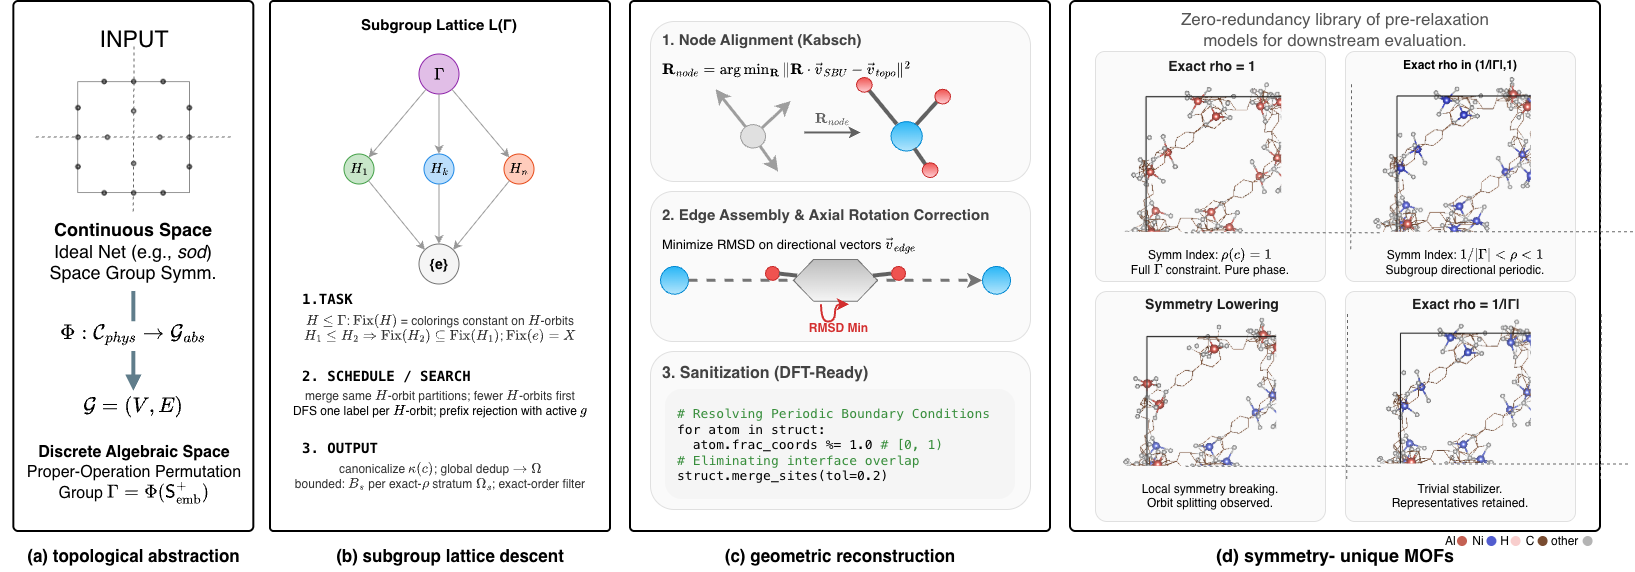
\includegraphics[width=\textwidth]{pipline.png}
    \caption{\textbf{Symmetry-aware candidate-generation pipeline.}}
    \label{fig:pipeline}
\end{figure}

\begin{algorithm}
\caption{Subgroup Lattice Descent}
\label{alg:enum}
\footnotesize
\begin{algorithmic}[1]
\Require Proper-rotation group $\Gamma$; vertex degrees $\{\deg(v)\}$; degree-typed ligand pools $\{\mathcal{C}_d\}$; degree counts $\{n_d\}$; optional task timeout $T_{\mathrm{task}}$; global cap $M_{\mathrm{total}}$; optional identity trigger $\Lambda_{\mathrm{id}}$ and identity cap $B_{\mathrm{id}}$
\Ensure Canonical representative set $\Omega$ with exact or partial Burnside report
\State initialize min-heap $Q$ keyed by orbit count; $\Omega \gets \emptyset$
\State push full-group task $\big(\mathcal{O}_{\Gamma},\,\infty\big)$ into $Q$
\For{each proper subgroup $H < \Gamma$ found from the subgroup lattice}
    \State compute $\mathcal{O}_H$ and its orbit-partition fingerprint
    \If{the fingerprint has not appeared before}
        \State push task $\big(\mathcal{O}_H,\,\infty\big)$ into $Q$
    \EndIf
\EndFor
\State $\mathcal{O}_{\{e\}} \gets \big\{\{v_1\},\dots,\{v_{|V|}\}\big\}$
\State estimate $\widehat{N}_{\mathrm{id}} \gets \text{naive-space} / |\Gamma|$
\State $b_{\mathrm{id}} \gets B_{\mathrm{id}}$ if $\widehat{N}_{\mathrm{id}} > \Lambda_{\mathrm{id}}$, else $\infty$
\State push identity task $\big(\mathcal{O}_{\{e\}},\,b_{\mathrm{id}}\big)$ into $Q$
\While{$Q$ is not empty}
    \State pop task $(\mathcal{O}, b)$ with smallest orbit count
    \State $s \gets |\Omega|$; deadline $\gets$ now $+\,T_{\mathrm{task}}$ if timeout is enabled
    \State \Call{CanonicalDFS}{$1,\; \langle \perp, \dots, \perp \rangle,\; \Gamma_{\mathrm{active}},\; \mathcal{O},\; b,\; s,\; \text{deadline}$}
\EndWhile
\State \Call{BurnsideReport}{$\Omega, \Gamma$} \Comment{exact closure or partial coverage}
\State \Return $\Omega$
\Statex
\Function{CanonicalDFS}{$k,\, c,\, \mathcal{A},\, \mathcal{O},\, b,\, s,\, \text{deadline}$}
    \If{deadline exceeded \textbf{ or } $|\Omega| \ge M_{\mathrm{total}}$ \textbf{ or } $|\Omega|-s \ge b$}
        \State \Return
    \EndIf
    \If{$k > |\mathcal{O}|$}
        \State $c^{\star} \gets \min_{g \in \Gamma} (g \cdot c)$
        \If{$c^{\star} \notin \text{Trie}$}
            \State insert $c^{\star}$; record $|\mathrm{Stab}_{\Gamma}(c^{\star})|$; $\Omega \gets \Omega \cup \{c^{\star}\}$
        \EndIf
        \State \Return
    \EndIf
    \State $d \gets \deg(\mathcal{O}_k)$
    \For{each $a \in \mathcal{C}_d$}
        \State assign $a$ to all vertices of $\mathcal{O}_k$
        \If{$\text{count}_d + |\mathcal{O}_k| > n_d$}
            \State undo $\mathcal{O}_k$; \textbf{continue}
        \EndIf
        \State $\mathcal{A}' \gets \emptyset$; $\;pruned \gets \textbf{false}$
        \For{each $g \in \mathcal{A}$}
            \If{$(g \cdot c) <_{lex} c$}
                \State $pruned \gets \textbf{true}$; \textbf{break}
            \ElsIf{$(g \cdot c) =_{lex} c$}
                \State $\mathcal{A}'.\text{add}(g)$
            \EndIf
        \EndFor
        \If{\textbf{not} $pruned$}
            \State \Call{CanonicalDFS}{$k+1,\, c,\, \mathcal{A}',\, \mathcal{O},\, b,\; s$}
        \EndIf
        \State undo assignment of $\mathcal{O}_k$
    \EndFor
\EndFunction
\end{algorithmic}
\end{algorithm}

\subsection*{From Enumerated Assignments to Crystal Models}
An enumerated assignment becomes a crystal model only after building-unit orientation is specified. The assignment is lifted to the periodic net, the unit-cell scale is set from the longest required connection length with a 5\% buffer, and directionality is recovered by two operations:
% 中文翻译：只有在指定构建单元取向之后，枚举指派才成为晶体模型。该指派先被提升回周期网络，晶胞尺度由最长所需连接长度加 5\% 缓冲确定，随后通过两个步骤恢复方向性：

\begin{enumerate}
\item \textbf{Node Alignment.} For each topological node, we collect the periodic connectivity vectors to all its neighbors.
The Kabsch algorithm then gives the optimal rotation matrix $\mathbf{R}_{node}$ for aligning the connection sites of the node SBU with these vectors, which fixes the spatial orientation of the SBU.
% 中文翻译：首先是“节点对齐”。对于每个拓扑节点，我们收集其与所有相邻节点之间的周期性连接向量。随后利用 Kabsch 算法求得最优旋转矩阵 $\mathbf{R}_{node}$，使节点构建单元（SBU）的连接位点与这些向量对齐，从而固定 SBU 的空间取向。

\item \textbf{Linker Placement.} For each edge in the graph, we compute the connection vector between two aligned nodes.
The algorithm retrieves the best-matching linker from the library, aligns it as a rigid body to this vector axis, and then refines its axial rotation by minimizing RMSD.
% 中文翻译：其次是“连接体放置”。对于图中的每条边，我们计算两个已对齐节点之间的连接向量。算法从库中检索最佳匹配的连接体，将其作为刚体对齐到该向量轴上，再通过最小化 RMSD 微调其绕轴旋转角度。
\end{enumerate}


After placement, coordinate normalization, lattice-aware edge adjustment, 0.8\,\AA\ X-site fusion, and near-duplicate merging handle periodic mismatches. A retained structure is a sanitizable periodic CIF: it passes deterministic CIF-format, reloadability, duplicate-site, and periodic-bookkeeping checks.
% 中文翻译：放置完成后，通过坐标归一化、考虑晶格周期性的边连接调整、0.8\,\AA\ X 位点融合和近重复位点合并处理周期性错位。被保留的结构即本文所说的可净化周期 CIF：它通过确定性的 CIF 格式、可重载性、重复位点和周期簿记检查。

Reconstruction treats each building unit as a rigid body. This is appropriate for SBUs with defined connection geometry and for linkers represented by one input conformer. The workflow does not perform conformational search. Section~\ref{sec:limits} states this boundary.
% 中文翻译：重构把每个构建单元视为刚体。该近似适用于具有明确连接几何的 SBU，以及由一个输入构象表示的连接体。该工作流不执行构象搜索。第~\ref{sec:limits}节说明这一边界。

\section*{Results}

We used the \texttt{ffc}, \texttt{fjh}, and \texttt{vba} nets as benchmark topologies because together they span small, larger, and beyond-exhaustive quotient-graph assignment spaces while retaining degree-compatible MOF building-unit placement.
% 中文翻译：本文采用 \texttt{ffc}、\texttt{fjh} 和 \texttt{vba} 网络作为基准拓扑，因为它们共同覆盖了小规模、较大规模以及超出完整穷举范围的商图指派空间，同时仍保持与 MOF 构建单元配位数相容的放置条件。

\subsection*{Algebraic Enumeration Checks}
Enumeration was checked by Burnside closure and CASM on identical quotient graphs (Table~\ref{tab:casm}). The \texttt{ffc} rows are exhaustive on both sides and provide the direct count check. The \texttt{fjh} rows compare exhaustive enumeration with matched bounded CASM runs, so they report larger-space coverage rather than exact-count disagreement.
% 中文翻译：枚举通过 Burnside 闭合以及同一商图上的 CASM 对照进行核对（表~\ref{tab:casm}）。\texttt{ffc} 行在双方均为可穷举运行，因此提供直接计数核对。\texttt{fjh} 行比较的是可穷举枚举器与匹配受限 CASM 运行，因此报告较大空间中的覆盖情况，而不是精确计数分歧。

\begin{table}[htbp]
\centering
\tiny
\setlength{\tabcolsep}{1.0mm}
\renewcommand{\arraystretch}{1.2}
\caption{CASM cross-checks on identical quotient graphs. Times are single-core wall-clock medians for the enumeration core.}
\label{tab:casm}
\begin{tabular}{llccccc}
\toprule
\textbf{Topology} & \textbf{Ligand pool} & \textbf{Naive} & \textbf{Orbits ($\Gamma$)} & \textbf{CASM} & \textbf{Undercount} & \textbf{Time ratio (s)} \\
\midrule
\texttt{ffc} & $|\mathcal{C}_3|{=}2,|\mathcal{C}_4|{=}2$ & $1.28\times10^{2}$ & 42      & 42      & 0\%  & $0.098 / 1.5\!\times\!10^{-4}$ \\
\texttt{ffc} & $|\mathcal{C}_3|{=}3,|\mathcal{C}_4|{=}3$ & $2.19\times10^{3}$ & 513     & 513     & 0\%  & $0.100 / 1.7\!\times\!10^{-3}$ \\
\midrule
\texttt{fjh} & $|\mathcal{C}_3|{=}1,|\mathcal{C}_4|{=}2$ & $4.10\times10^{3}$ & 394     & 265     & 33\% & $0.194 / 3.3\!\times\!10^{-3}$ \\
\texttt{fjh} & $|\mathcal{C}_3|{=}2,|\mathcal{C}_4|{=}1$ & $6.55\times10^{4}$ & 4{,}756 & 2{,}476 & 48\% & $0.291 / 0.057$ \\
\texttt{fjh} & $|\mathcal{C}_3|{=}1,|\mathcal{C}_4|{=}3$ & $5.31\times10^{5}$ & 36{,}369& 20{,}655& 43\% & $2.12 / 0.402$ \\
\bottomrule
\end{tabular}
\end{table}

For bounded \texttt{vba} runs, current safeguards returned 131{,}864 orbits from $4.29\times10^{9}$ assignments (0.026\%) for $|\mathcal{C}_4|{=}2$ and 500{,}000 orbits from $1.85\times10^{15}$ assignments ($<0.001\%$) for $|\mathcal{C}_4|{=}3$. These outputs are symmetry-prioritized prefixes, not exhaustive counts.
% 中文翻译：对于受限 \texttt{vba} 运行，当前保护机制在 $|\mathcal{C}_4|{=}2$ 时从 $4.29\times10^{9}$ 个指派中返回 131{,}864 个轨道（0.026\%），在 $|\mathcal{C}_4|{=}3$ 时从 $1.85\times10^{15}$ 个指派中返回 500{,}000 个轨道（$<0.001\%$）。这些输出是按对称性优先排序的前缀，而不是可穷举计数。
\subsection*{Geometric Instantiation Across Representative Topologies}
\label{sec:validation}

We next tested whether accepted assignments could be reconstructed as periodic frameworks. Figure~\ref{fig:reconstruction_gallery} gives representative models, while Table~\ref{tab:reconstruction_audit} reports the quantitative audit for sampled \texttt{ffc} and \texttt{fjh} candidates.
% 中文翻译：随后检验被接受的指派能否重构为周期性框架。图~\ref{fig:reconstruction_gallery} 给出代表模型，表~\ref{tab:reconstruction_audit} 报告抽样 \texttt{ffc} 和 \texttt{fjh} 候选的定量审计。


\begin{figure}[p]
    \centering
    \begin{subfigure}[t]{0.49\linewidth}
        \centering
        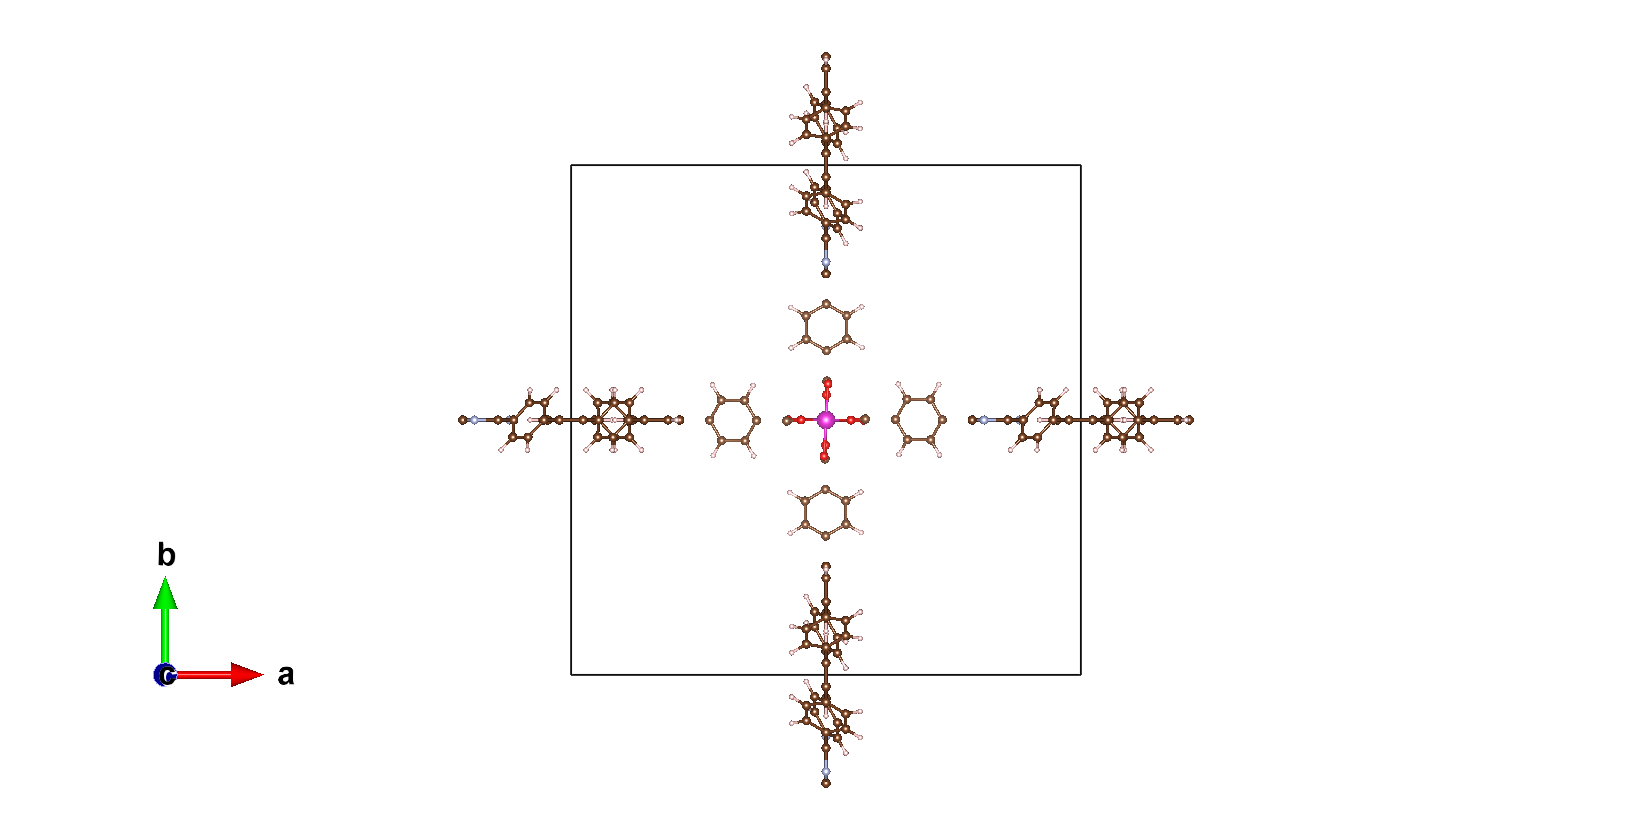
\includegraphics[width=\linewidth,trim={130bp 35bp 420bp 35bp},clip]{ffc_comp_b_21.png}
        \caption*{\texttt{ffc}}
    \end{subfigure}
    \hfill
    \begin{subfigure}[t]{0.49\linewidth}
        \centering
        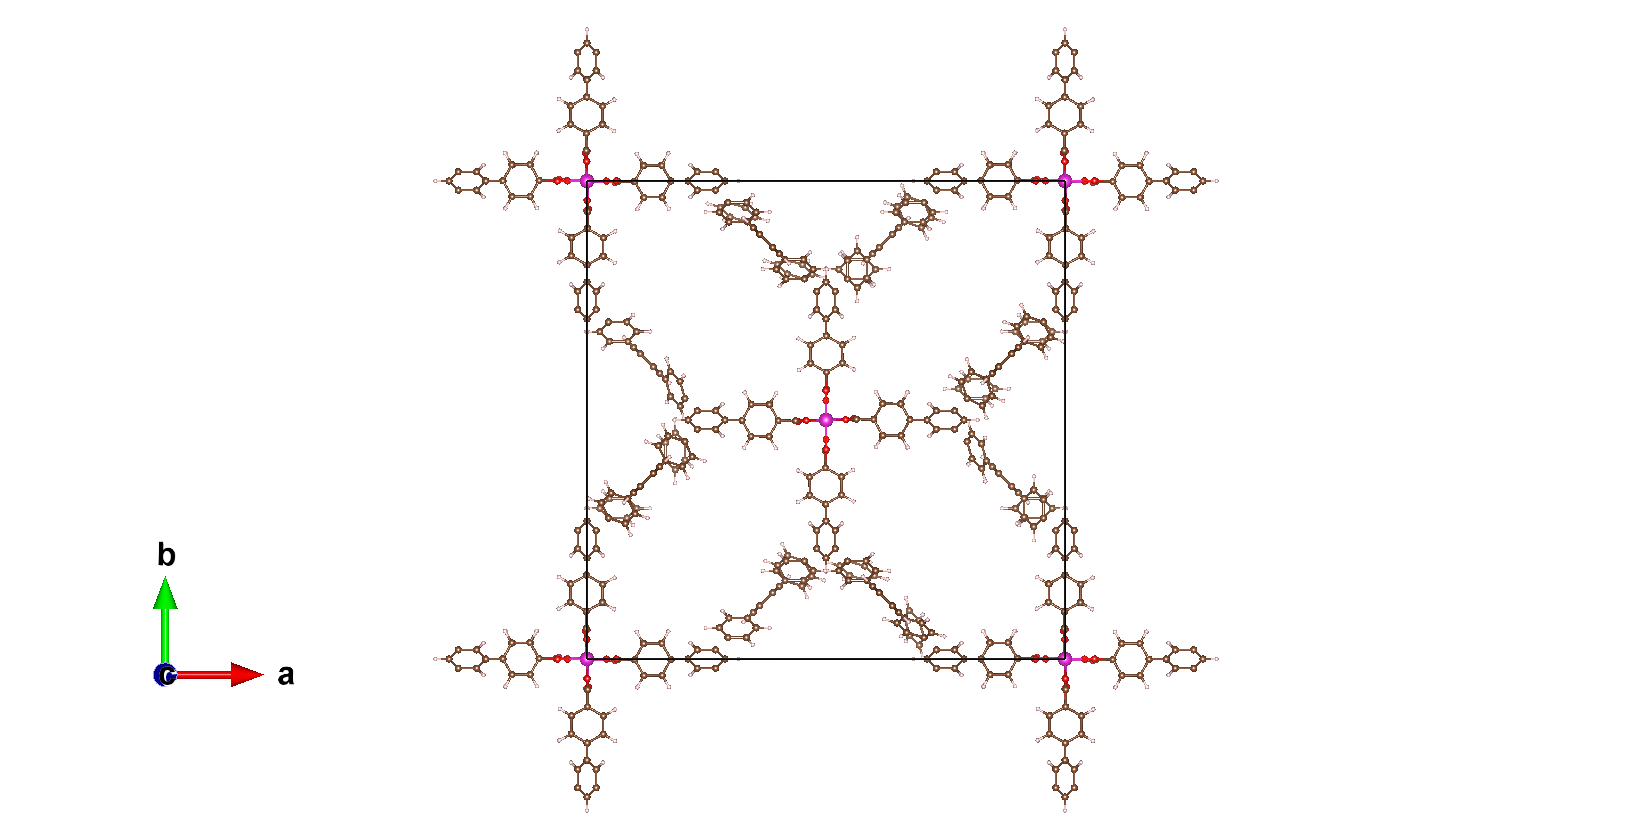
\includegraphics[width=\linewidth,trim={130bp 20bp 400bp 20bp},clip]{fjh_comp_b_1.png}
        \caption*{\texttt{fjh}}
    \end{subfigure}

    \vspace{0.75em}

    \begin{subfigure}[t]{0.72\linewidth}
        \centering
        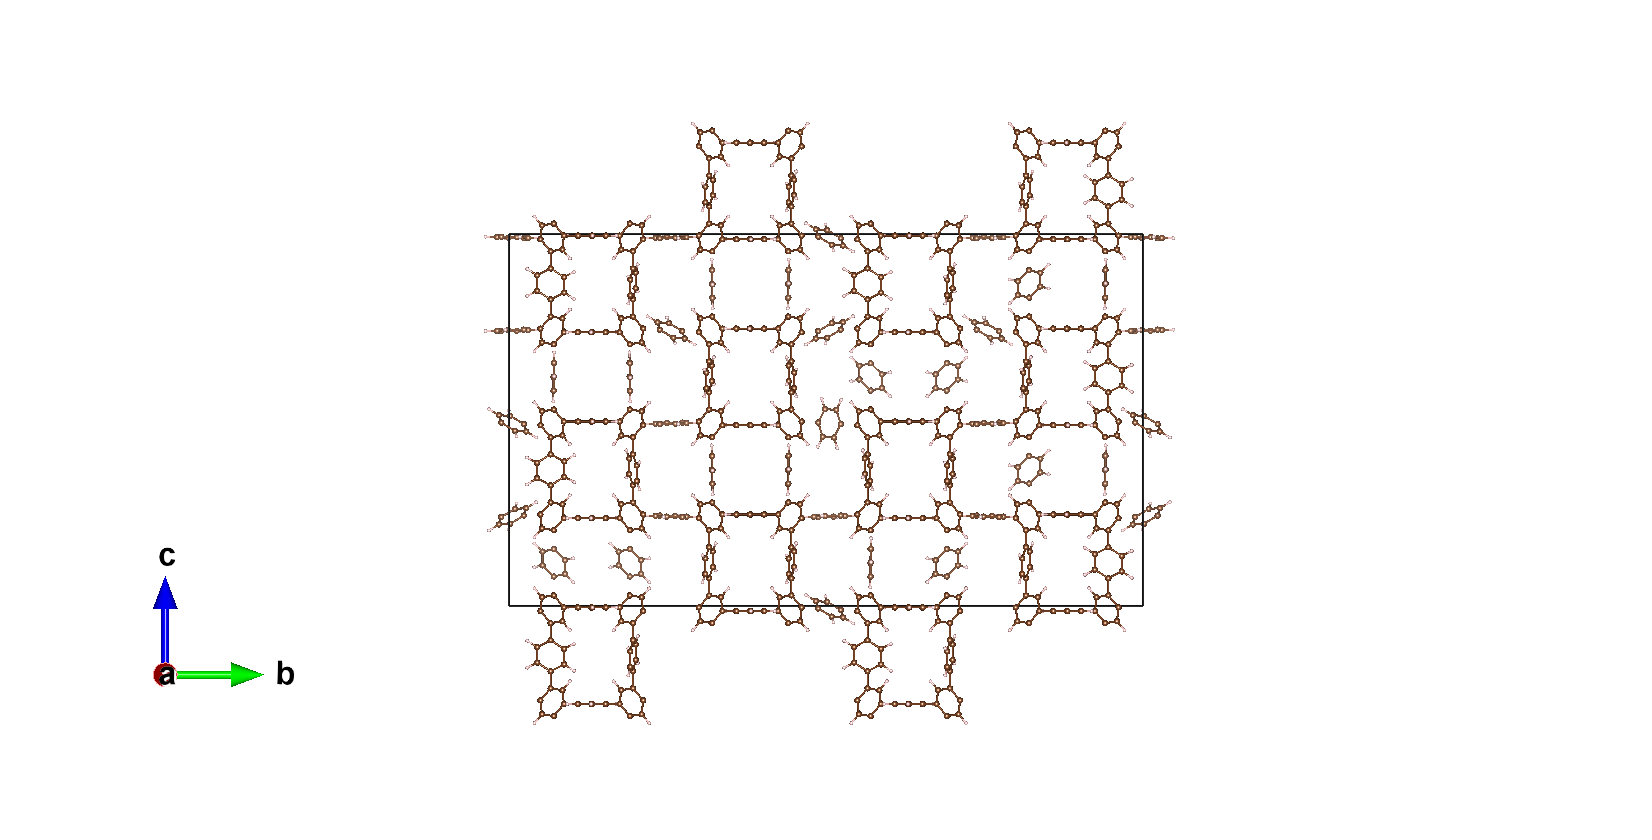
\includegraphics[width=\linewidth,trim={130bp 90bp 435bp 90bp},clip]{vba_rho1.png}
        \caption*{\texttt{vba}}
    \end{subfigure}
    \caption{Representative pre-relaxation crystal models reconstructed from symmetry-distinct assignments in \texttt{ffc}, \texttt{fjh}, and \texttt{vba}.}
    % 中文翻译：由 \texttt{ffc}、\texttt{fjh} 和 \texttt{vba} 中的对称互异指派重构得到的代表性弛豫前晶体模型。
    \label{fig:reconstruction_gallery}
\end{figure}

\begin{table}[htbp]
\centering
\caption{\textbf{Reconstruction audit for sampled \texttt{ffc} and \texttt{fjh} pre-relaxation starting models.}}
% 中文翻译：抽样 \texttt{ffc} 和 \texttt{fjh} 弛豫前起始模型的重构审计。
\label{tab:reconstruction_audit}
\begin{tabular}{lccccc}
\toprule
Topology & Attempted & Assembled & Sanitizable CIF & Topology-pass & Clash-free \\
\midrule
\texttt{ffc} & 12 & 12/12 & 12/12 & 12/12 & 12/12 \\
\texttt{fjh} & 15 & 15/15 & 15/15 & 15/15 & 15/15 \\
\midrule
Combined & 27 & 27/27 & 27/27 & 27/27 & 27/27 \\
\bottomrule
\end{tabular}
\end{table}


\subsection*{Illustrative Screening-Stage DFT Example}

We evaluated single-point density functional theory (DFT) energies for rigidly assembled structures within fixed chemical compositions. The structures were not relaxed, so all energy differences refer to the same assembled-geometry basis.
% 中文翻译：我们对固定化学组成内的刚性组装结构计算了单点密度泛函理论（DFT）能量。结构未进行弛豫，因此所有能量差异均对应同一组装几何基准。

For \texttt{ffc}, 21 converged calculations span eight fixed-composition groups. Using the bins low $[0,0.25)$, medium $[0.25,0.75]$, and high $(0.75,1]$, every composition-wise minimum falls in the medium- or high-symmetry strata (Fig.~\ref{fig:symmetry_screening}).
% 中文翻译：对于 \texttt{ffc}，21 个已收敛计算分布在 8 个固定组成组中。按低对称 $[0,0.25)$、中对称 $[0.25,0.75]$ 和高对称 $(0.75,1]$ 划分时，每个组成组的最低能点均落在中对称或高对称层级（图~\ref{fig:symmetry_screening}）。

For \texttt{fjh}, two completed fixed-composition sets each contain 16 converged calculations across five $\rho$ strata. Their minima occur at $\rho=0.5$ for \texttt{comp\_a} and $\rho=1.0$ for \texttt{comp\_b}. Together with \texttt{ffc}, these tests indicate that the symmetry-prioritized traversal includes low-energy structures in the sampled screening space~\cite{peng2024learning,zeni2023mattergen,okabe2025structural}.
% 中文翻译：对于 \texttt{fjh}，两个已完成固定组成集合各包含 16 个已收敛计算，并覆盖 5 个 $\rho$ 层级。最低能点分别出现在 \texttt{comp\_a} 的 $\rho=0.5$ 和 \texttt{comp\_b} 的 $\rho=1.0$。结合 \texttt{ffc} 结果，这些测试表明对称性优先遍历在当前采样筛选空间中包含低能结构~\cite{peng2024learning,zeni2023mattergen,okabe2025structural}。


\begin{figure}[htbp]
    \centering
    \begin{subfigure}[t]{0.495\linewidth}
        \centering
        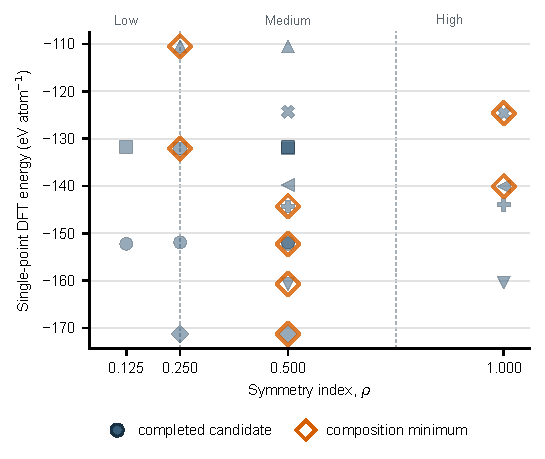
\includegraphics[width=\linewidth]{ffc_pooled_symmetry_energy_a.pdf}
        \caption{Pooled single-point energies for the \texttt{ffc} set.}
    \end{subfigure}
    \hfill
    \begin{subfigure}[t]{0.495\linewidth}
        \centering
        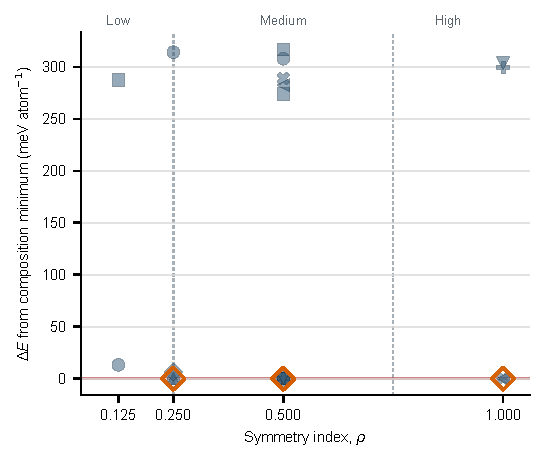
\includegraphics[width=\linewidth]{ffc_pooled_symmetry_energy_b.pdf}
        \caption{Composition-controlled $\Delta E$ for the same \texttt{ffc} candidates.}
    \end{subfigure}
    
    \vspace{0.5em}

    \begin{subfigure}[t]{0.495\linewidth}
        \centering
        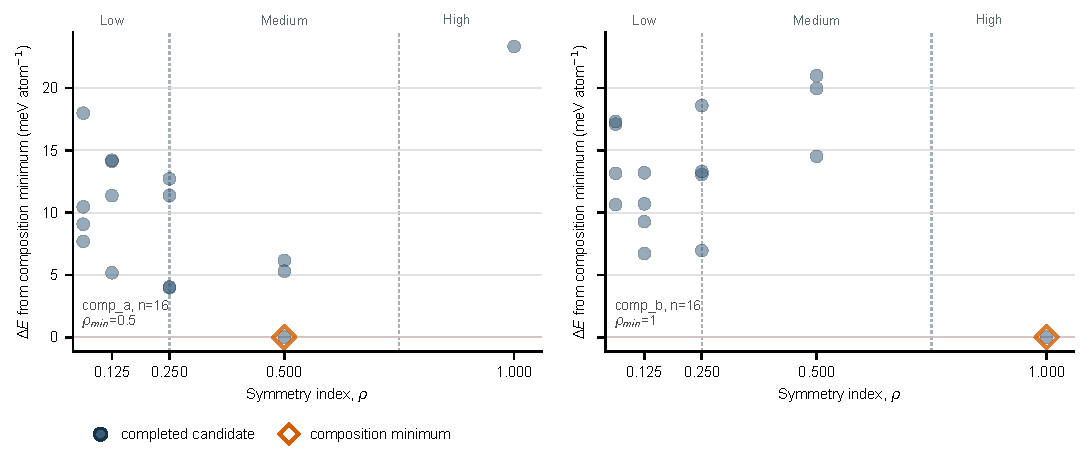
\includegraphics[width=\linewidth,trim={0 0 262 0},clip]{fjh_dual_delta_symmetry_energy.pdf}
        \caption{\texttt{fjh comp\_a} composition-controlled $\Delta E$.}
    \end{subfigure}
    \hfill
    \begin{subfigure}[t]{0.495\linewidth}
        \centering
        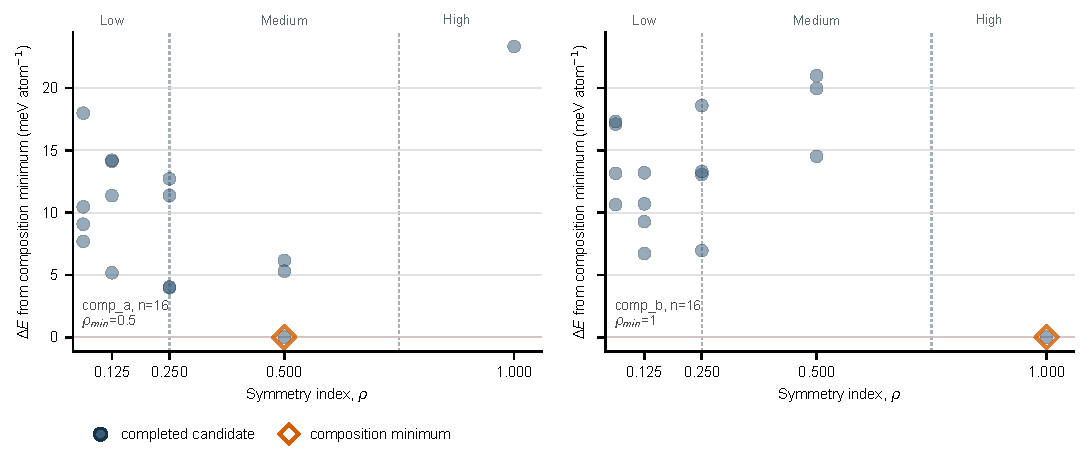
\includegraphics[width=\linewidth,trim={262 0 0 0},clip]{fjh_dual_delta_symmetry_energy.pdf}
        \caption{\texttt{fjh comp\_b} composition-controlled $\Delta E$.}
    \end{subfigure}
\caption{Illustrative single-point DFT screening results across two topology scales. Filled markers denote converged candidates; open markers denote fixed-composition minima.}
% 中文翻译：两种拓扑尺度下的说明性单点 DFT 筛选结果。实心标记表示已收敛候选，空心标记表示固定组成比较中的最低能点。
    \label{fig:symmetry_screening}
\end{figure}

\subsection*{Matched Ordering Check for CO$_2$/N$_2$ Screening}

We also tested whether fixed-composition orderings can differ in a gas-separation screen. Existing \texttt{ffc} CO$_2$/N$_2$ labels were grouped with composition, $\rho$, and symmetry stratum fixed within each comparison.
% 中文翻译：我们还检验固定组成排布是否会在气体分离筛选中产生差异。已有 \texttt{ffc} CO$_2$/N$_2$ 标签按比较组整理，并在组内固定组成、$\rho$ 和对称层级。

Table~\ref{tab:ffc_co2n2_ordering} summarizes three matched groups. Within each group, ordering changes altered pore descriptors and GCMC-derived labels. These labels are screening-stage responses for as-assembled starting models.
% 中文翻译：表~\ref{tab:ffc_co2n2_ordering} 汇总了 3 个匹配比较组。在每个组内，排布变化会改变孔结构描述符和 GCMC 派生标签。这些标签只是组装初始模型的筛选阶段响应。

\begin{table}[htbp]
\centering
\scriptsize
\caption{\textbf{Matched \texttt{ffc} ordering check using CO$_2$/N$_2$ screening labels.} Ranges summarize four symmetry-distinct orderings per fixed-composition group.}
% 中文翻译：使用 CO$_2$/N$_2$ 筛选标签进行的匹配 \texttt{ffc} 排布检查。范围值汇总每个固定组成组内的 4 个对称互异排布。
\label{tab:ffc_co2n2_ordering}
\setlength{\tabcolsep}{1.0mm}
\renewcommand{\arraystretch}{1.12}
\begin{tabular}{@{}lccccccc@{}}
\toprule
\textbf{Group} & \textbf{$n$} & \textbf{$\rho$/stratum} & \textbf{PLD (\AA)} & \textbf{LCD (\AA)} & \textbf{WC} & \textbf{S} & \textbf{APS} \\
\midrule
A & 4 & 0.25/Med & 27.39--28.27 & 26.41--27.07 & 0.345--0.411 & 1.948--2.188 & 0.595--0.817 \\
B & 4 & 0.50/High & 27.36--27.79 & 26.15--26.83 & 0.341--0.386 & 1.923--2.187 & 0.588--0.760 \\
C & 4 & 0.50/High & 27.31--27.78 & 25.80--26.81 & 0.349--0.422 & 1.981--2.208 & 0.626--0.839 \\
\bottomrule
\end{tabular}
\end{table}



\section*{Discussion}
\label{sec:discussion}
The workflow couples non-redundant enumeration to reconstruction-ready models. Exact Burnside/CASM checks support the orbit-counting logic for the exhaustive \texttt{ffc} cases, and bounded \texttt{vba} runs show how the same scheduler behaves beyond the exhaustive range. The sampled \texttt{ffc}/\texttt{fjh} audit then checks whether retained assignments can be written as sanitizable, topology-consistent, clash-free CIFs.
% 中文翻译：该工作流把无冗余枚举与可重构模型相连接。精确 Burnside/CASM 核对支撑可穷举 \texttt{ffc} 算例中的轨道计数逻辑，受限 \texttt{vba} 运行说明同一调度器在超出可穷举范围后的行为。随后，抽样 \texttt{ffc}/\texttt{fjh} 审计检验保留指派能否写成可净化、拓扑一致且无短接触警告的 CIF。

The DFT and CO$_2$/N$_2$ examples test the interface to downstream screening. They indicate that reconstructed sets can be scored under fixed-composition controls and that ordered assignments can carry different screening labels. This is the crystal-engineering relevance of the ordering step: arrangement becomes a controlled variable before expensive evaluation, rather than an accidental duplicate in a generated database. These examples support candidate preparation, not final material ranking.
% 修改点：晶体工程意义移到 Discussion，由结果支撑，而不是在 Introduction 里提前判断。
% 中文翻译：DFT 和 CO$_2$/N$_2$ 示例检验该流程与下游筛选的接口。它们说明重构集合可以在固定组成控制下打分，且有序指派可携带不同筛选标签。这正是排布步骤的晶体工程意义：排布在高成本评估之前成为受控变量，而不是生成数据库中的偶然重复项。这些示例支撑的是候选准备，而不是最终材料排序。

\subsection*{Current Limits of the Validation}
\label{sec:limits}
The main model limit is rigid-body reconstruction. The implementation assumes that node SBUs and linkers can be placed as rigid units once connection geometry is specified. It therefore tests fixed-conformer geometric compatibility, not flexible-framework conformational space. The DFT results are single-point scores on as-assembled structures, and the CO$_2$/N$_2$ labels come from one screening protocol. Neither replaces relaxation, thermodynamic ranking, or longer adsorption studies.
% 中文翻译：主要模型限制来自刚体重构。当前实现假定节点 SBU 和连接体在连接几何给定后可作为刚性单元放置。因此，它检验的是固定构象几何相容性，而不是柔性框架的构象空间。DFT 结果是组装初始结构的单点分数，CO$_2$/N$_2$ 标签来自一个筛选协议。二者都不能替代弛豫、热力学排序或更完整的吸附研究。

The implementation also assumes a single primitive quotient graph and one embedded net. It does not automatically generate interpenetrated frameworks, multiple independent nets, or supercell colorings. These cases require explicit multi-net or supercell inputs. Distinct enumerated assignments may also relax into similar or identical geometries, so post-relaxation identity remains a separate validation step.
% 中文翻译：当前实现还假定输入为单个初基商图和一个嵌入网络。它不会自动生成互穿框架、多个独立网络或超胞着色。这些情形需要显式的多网络或超胞输入。不同枚举指派也可能在弛豫后收敛到相似或相同几何，因此弛豫后的同一性仍是独立验证步骤。

\section*{Conclusion}
This work describes a deterministic route from fixed topological MOF design spaces to symmetry-distinct, oriented candidate models. Proper-rotation orbit enumeration removes reconstruction-compatible redundancy, and rigid-body Kabsch alignment converts retained assignments into periodic models with explicit building-unit orientation.
% 中文翻译：本文描述了一条确定性路线，将固定拓扑 MOF 设计空间转化为对称互异、具有取向信息的候选模型。真旋转轨道枚举去除与重构相容的冗余，刚体 Kabsch 对齐把保留指派转化为具有显式构建单元取向的周期模型。

The evidence supports that route within a defined scope: exhaustive orbit checks, sampled reconstruction audits, and screening-stage DFT and CO$_2$/N$_2$ examples. The deposited CIFs are pre-relaxation starting models. Subsequent relaxation, adsorption or electronic-structure screening, and active selection should test which candidates remain distinct and useful after higher-cost evaluation.
% 中文翻译：本文证据在明确范围内支撑这一路线：可穷举轨道核对、抽样重构审计，以及筛选阶段 DFT 和 CO$_2$/N$_2$ 示例。存放的 CIF 是弛豫前起始模型。后续弛豫、吸附或电子结构筛选以及主动选择应进一步检验哪些候选在高成本评估后仍保持互异且有用。

\section*{Methods}
\subsection*{Computational Details}
The framework is implemented in Python 3.8. It follows three stages: symmetry extraction on the periodic net, symmetry-distinct enumeration on the quotient graph, and rigid-body reconstruction of accepted assignments.
% 中文翻译：该框架基于 Python 3.8 实现，包含三个阶段：周期网络对称性提取、商图上的对称互异枚举，以及被接受指派的刚体重构。

Inputs are a primitive quotient graph, one chosen net embedding, and degree-compatible building-unit pools. Benchmark topologies were taken from net embeddings associated with the Reticular Chemistry Structure Resource (RCSR)~\cite{okeeffe2008rcsr}. The method removes redundant building-block assignments within this fixed input; it does not benchmark global net classification or cross-database colored-net equivalence.
% 中文翻译：输入包括初基商图、一个选定网络嵌入以及配位数相容的构建单元库。基准拓扑来自与网状化学结构资源（RCSR）关联的网络嵌入~\cite{okeeffe2008rcsr}。该方法只在固定输入内去除冗余 building-block 指派，不对全局网络分类或跨数据库 colored-net 等价性做基准。

In Phase I, \texttt{pymatgen} is used for crystallographic symmetry analysis. We scan \texttt{symprec} $\in \{0.01, 0.1, 0.3\}$\,\AA\ and project consistent operations onto graph automorphism groups.
% 中文翻译：第一阶段使用 \texttt{pymatgen} 进行晶体学对称性分析。我们扫描 \texttt{symprec} $\in \{0.01, 0.1, 0.3\}$\,\AA，并将一致的操作投影为图自同构群。

In Phase II, proper subgroups are traversed with a SymPy-based lattice walk and a cyclic-subgroup fallback. Orbit calculations, canonical checks, and duplicate removal use compact data structures. Optional safeguards include per-task timeouts and global caps.
% 中文翻译：第二阶段通过基于 SymPy 的子群格搜索遍历真子群，并设置循环子群回退路径。轨道计算、正则形检查和去重使用紧凑数据结构。可选保护机制包括任务超时和全局数量上限。

In Phase III, the Kabsch algorithm is implemented by singular value decomposition in \texttt{NumPy}. The assembled structure then undergoes secondary symmetry analysis with \texttt{symprec}=0.3\,\AA.
% 中文翻译：第三阶段通过 \texttt{NumPy} 奇异值分解实现 Kabsch 算法。组装结构随后以 \texttt{symprec}=0.3\,\AA 进行二次对称性分析。

The reconstruction sequence is graph enrichment, rigid-body node/linker placement, periodic coordinate normalization, and sanitization before downstream screening.
% 中文翻译：重构顺序为图信息增强、节点/连接体刚体放置、周期性坐标归一化，以及下游筛选前的净化。

All computations were executed on a single-core Intel Core i5 processor.
% 中文翻译：所有计算均在单核 Intel Core i5 处理器上执行。

The main-text validation cases used \texttt{3c\_B\_Ch}, \texttt{3c\_triazine\_Ch}, \texttt{4c\_B\_Ch}, \texttt{4c\_Cd\_1\_Ch}, \texttt{4c\_Cu\_1\_Ch}, and \texttt{1B\_4H\_Ch}. Full inventories and CIF files are provided in the data package. Cd is the primary closed-shell metal node in the reported \texttt{ffc}/\texttt{fjh} DFT sets; Cu appears in optional open-shell probe or visual-example pools.
% 中文翻译：主文验证算例使用 \texttt{3c\_B\_Ch}、\texttt{3c\_triazine\_Ch}、\texttt{4c\_B\_Ch}、\texttt{4c\_Cd\_1\_Ch}、\texttt{4c\_Cu\_1\_Ch} 和 \texttt{1B\_4H\_Ch}。完整清单和 CIF 文件见数据包。Cd 是报告的 \texttt{ffc}/\texttt{fjh} DFT 集合中的主要闭壳金属节点；Cu 出现在可选开壳探针或可视化示例池中。

\subsection*{CASM Comparison Protocol}

Cross-validation uses \textsf{libcasm-configuration}~2.3.1 and \textsf{libcasm-xtal}~2.3.0 under Python~3.11. CASM receives the same degree-constrained quotient graph, with each site assigned the occupant set allowed by its coordination number. A run is accepted only when the proper-rotation subgroup of the CASM factor group has the same order $|\Gamma|$. Primitive-cell enumeration gives one representative per full-group orbit, which is reconciled to the proper-rotation count $P=A+2C$. Each timing is the median of three isolated single-thread subprocess runs. \texttt{vba} CASM attempts were stopped by a wall-clock or memory watchdog.
% 中文翻译：交叉验证在 Python~3.11 下使用 \textsf{libcasm-configuration}~2.3.1 和 \textsf{libcasm-xtal}~2.3.0。CASM 接收相同的度数约束商图，每个位点的占据集合由其配位数决定。仅当 CASM 因子群的真旋转子群阶与 $|\Gamma|$ 一致时，才接受该运行。初基胞枚举给出每个全群轨道的一个代表元，并通过 $P=A+2C$ 对账到真旋转计数。计时为三个隔离单线程子进程运行的中位数。\texttt{vba} CASM 尝试由墙钟或内存看门狗停止。

\subsection*{DFT Energy Validation}
Single-point energies were computed with CP2K/Quickstep~\cite{cp2k2020} using PBE+D3~\cite{perdew1996pbe,grimme2010d3}, DZVP-MOLOPT-PBE-GTH basis sets, GTH pseudopotentials, and 500/60\,Ry plane-wave/relative cutoffs. Self-consistent field (SCF) calculations used diagonalization, Fermi--Dirac smearing at 300\,K, 30 added molecular orbitals, Broyden charge mixing, $\mathrm{EPS\_SCF}=5\times10^{-5}$, and a 300-step ceiling.
% 中文翻译：单点能通过 CP2K/Quickstep~\cite{cp2k2020} 计算，采用 PBE+D3~\cite{perdew1996pbe,grimme2010d3}、DZVP-MOLOPT-PBE-GTH 基组、GTH 赝势，以及 500/60\,Ry 的平面波/相对截断能。自洽场（SCF）计算使用对角化、300\,K Fermi--Dirac 展宽、30 个附加分子轨道、Broyden 电荷混合、$\mathrm{EPS\_SCF}=5\times10^{-5}$ 和 300 步上限。

Energy comparisons were made only within fixed compositions on rigidly assembled geometries. The \texttt{ffc} set contains 21 converged calculations across eight composition groups. The completed \texttt{fjh comp\_a} and \texttt{fjh comp\_b} subsets contain 32 converged structures across two independent fixed-composition tests. Reported energies are geometry-consistent screening scores; thermodynamic ranking requires later relaxation.
% 中文翻译：能量比较只在固定组成内部、基于刚性组装几何进行。\texttt{ffc} 集合包含 8 个组成组中的 21 个已收敛计算；已完成的 \texttt{fjh comp\_a} 和 \texttt{fjh comp\_b} 子集在两个独立固定组成测试中共包含 32 个已收敛结构。报告能量是几何一致的筛选阶段分数；热力学排序需要后续弛豫。

\subsection*{CO$_2$/N$_2$ Screening Labels}
The matched ordering check used existing \texttt{ffc} clean-pool CO$_2$/N$_2$ labels. We selected three fixed-composition groups, each with four symmetry-distinct orderings at the same $\rho$ and stratum. Pore-limiting and largest-cavity diameters were computed with Zeo++~\cite{willems2012algorithms}.
% 中文翻译：匹配排布检查使用已有 \texttt{ffc} clean-pool CO$_2$/N$_2$ 标签。我们选取 3 个固定组成组，每组含 4 个具有相同 $\rho$ 和层级的对称互异排布。孔限制直径和最大孔腔直径由 Zeo++ 计算~\cite{willems2012algorithms}。

Grand canonical Monte Carlo labels were generated with RASPA2~\cite{dubbeldam2016raspa} for dry CO$_2$/N$_2$ screening~\cite{altintas2018database}. Simulations used 0.15/0.85 gas mole fractions at 298\,K, 1.0/0.1\,bar adsorption/desorption pressures, CIF-derived charges, \texttt{ExampleMOFsForceField}, \texttt{ExampleDefinitions}, \texttt{UnitCells 1 1 1}, 10000 Monte Carlo cycles, and 5000 initialization cycles. Metrics were $S=(q_{\mathrm{CO_2}}/q_{\mathrm{N_2}})/(y_{\mathrm{CO_2}}/y_{\mathrm{N_2}})$, $WC=q_{\mathrm{CO_2}}(1.0\,\mathrm{bar})-q_{\mathrm{CO_2}}(0.1\,\mathrm{bar})$, $R=WC/q_{\mathrm{CO_2}}(1.0\,\mathrm{bar})$, and $APS=S\times WC\times R$.
% 中文翻译：巨正则蒙特卡洛标签由 RASPA2 生成~\cite{dubbeldam2016raspa}，用于干态 CO$_2$/N$_2$ 筛选~\cite{altintas2018database}。模拟采用 0.15/0.85 气相摩尔分数、298\,K、1.0/0.1\,bar 吸附/脱附压力、CIF 电荷、\texttt{ExampleMOFsForceField}、\texttt{ExampleDefinitions}、\texttt{UnitCells 1 1 1}、10000 个蒙特卡洛循环和 5000 个初始化循环。指标为 $S=(q_{\mathrm{CO_2}}/q_{\mathrm{N_2}})/(y_{\mathrm{CO_2}}/y_{\mathrm{N_2}})$、$WC=q_{\mathrm{CO_2}}(1.0\,\mathrm{bar})-q_{\mathrm{CO_2}}(0.1\,\mathrm{bar})$、$R=WC/q_{\mathrm{CO_2}}(1.0\,\mathrm{bar})$ 和 $APS=S\times WC\times R$。

\section*{Data availability}
The code and supporting data are publicly available at GitHub: https://github.com/Buct454/mof-enumeration-reconstruction.git. The package includes representative CIFs for Fig.~\ref{fig:reconstruction_gallery}, sampled \texttt{ffc}/\texttt{fjh} CIFs and reconstruction audit tables for Table~\ref{tab:reconstruction_audit}, and the CO$_2$/N$_2$ ordering CSV with 12 candidate labels. Deposited CIFs are pre-relaxation starting models with validation metadata, not relaxed crystal structures.
% 中文翻译：代码和支撑数据已公开存放于 GitHub：https://github.com/Buct454/mof-enumeration-reconstruction.git。数据包包括图~\ref{fig:reconstruction_gallery} 的代表性 CIF、支撑表~\ref{tab:reconstruction_audit} 的抽样 \texttt{ffc}/\texttt{fjh} CIF 和重构审计表，以及包含 12 个候选标签的 CO$_2$/N$_2$ 排布 CSV。存放的 CIF 是带验证元数据的弛豫前起始模型，不是已弛豫晶体结构。

\section*{Acknowledgements}
This work was supported by the National Key R\&D Program of China (No. 2021YFB3802200).

\section*{Author Contributions}
H.L. conceived the study. H.L. and J.T. developed the algorithm, implemented the workflow, and performed the computational experiments. D.L., M.T., and Q.Y. contributed to method discussion, result interpretation, and manuscript refinement. All authors discussed the results, reviewed the manuscript, and approved the final version.
% 中文翻译：H.L. 构思了本研究。H.L. 和 J.T. 开发了算法、实现了工作流程并完成了计算实验。D.L.、M.T. 和 Q.Y. 参与了方法讨论、结果解释和手稿完善。所有作者讨论了研究结果、审阅了手稿并批准了最终版本。


\section*{Competing Interests}
The authors declare that they have no competing financial interests, personal relationships, or other conflicts of interest that could have influenced the work reported in this manuscript.
% 中文翻译：作者声明不存在可能影响本文工作的竞争性经济利益、个人关系或其他利益冲突。



\newpage
\clearpage

\bibliography{reference}

\end{document}
